\documentclass[twocolumn]{article}
\usepackage[margin=0.7in]{geometry}
\usepackage{graphicx}
\usepackage{url}

%opening
\title{One-Dimensional Interior Models of Europa}
\author{Isabelle Joosten\\Student number 4998480\\Assignment 1 for the course ``Physics of Planetary Interiors" (AE4893-24)\\Total time spent: 44 hours}

\begin{document}

\maketitle

\section{Introduction}
Europa is one of Jupiter's largest moons. It is an interesting planetary body because it is commonly thought to have a subsurface liquid water ocean that may be capable of harbouring life. In this report, various models of Europa's interior found in literature are analysed and compared. Based on those, three new models are constructed, with the aim to characterise the global interior of the icy moon.

\section{Literature Study}
Several existing models of Europa's interior were consulted for the purposes of this assignment. Jin and Ji\cite{jinInternalStructureModels2012} published an article in which they outline the creation of 3 models of Europa, the difference between the models being the assumed composition of the core: Fe, FeS, or Fe\textsubscript{0.8}(FeS)\textsubscript{0.2}. Aside from the core, Jin and Ji define two more layers in each of their models: an olivine mantle and an outer shell made of water. To generate interior profiles of Europa, they choose a fractional mass for each of the 3 layers as well as a centre pressure. The program they developed performs an integration from the centre to the surface in order to solve for the surface pressure, logically must be 0. Based on the calculated surface pressure, the program then adjusts the centre pressure before restarting the integration, repeating this sequence until the calculated surface pressure is 0.\\
Another existing model found in literature is one published by Cammarano et al.\cite{cammaranoLongperiodSeismologyEuropa2006}. The aim of their research was to find the seismic velocities associated with different possible interior of Europa, so their model determines the density profile based on temperature and composition. Like Jin and Ji, Cammarano et al. assume an FeS core and a water shell, but unlike Jin and Ji, they consider two different mantle compositions: pyrolitic and chondritic.\\
Kuskov and Kronrod\cite{kuskovInternalStructureEuropa2005} base their model on the observed mass, bulk density, and moment of inertia of Europa. Unlike the two models perviously discussed in this section, in this model the mantle is divided into 3 layers, leading to 5 layers in total.\\
Finally, Howell\cite{howellLikelyThicknessEuropas2021} focuses on Europa's icy outer shell, and attempts to determine the thickness of this shell based on its steady-state heat flux. This model differs from the others in that it does not provide a profile of Europa's full interior, but rather provides a detailed profile of the ice crust based on assumed values for the rest of the interior.\\
Because all models found use a different approach and were created with a different goal in mind, a direct comparison is difficult to make. Nevertheless, there are a few notable trends among the articles. There seems to be a general consensus among researchers that Europa consists of an iron-rich core, a silicate or chondritic mantle, and an ice/water outer shell\footnote{It should be noted, though, that this is by no means definitively proven. See for example Trinh et al.\cite{trinhSlowEvolutionEuropas2023}, in which the existence of Europa's metallic core is questioned based on reanalysis of Galileo data.}. Numerically, there is some variation between the outputs of each model, part of which can be explained by the fact that the models use different theoretical values as inputs, most of which are, themselves, obtained through theoretical modeling\footnote{A frequently cited paper in literature about Europa's interior is Anderson et al. (1998)\cite{andersonEuropasDifferentiatedInternal1998}, which is where a lot of input values are taken from. Unfortunately, this article appears to be behind a paywall.}. A summary of relevant values is given in Table \ref{tab:modelcomparison}. As each of these models has undergone some form of verification and validation before being published, these values, or averages thereof, will be used as reference values for the remainder of this report.

% Please add the following required packages to your document preamble:
% \usepackage{graphicx}
% Please add the following required packages to your document preamble:
% \usepackage{graphicx}
\begin{table*}[h]
	\caption{An overview of the models analysed for this assignment.}
	\label{tab:modelcomparison}
	\resizebox{\textwidth}{!}{%
		\begin{tabular}{l|llll}
			& \textbf{Jin and Ji}         & \textbf{\begin{tabular}[c]{@{}l@{}}Cammarano\\ et al.\end{tabular}} & \textbf{\begin{tabular}[c]{@{}l@{}}Kuskov\\ and Kronrod\end{tabular}} & \textbf{Howell}              \\ \hline
			\textbf{Total radius {[}km{]}}     & 1563                        & Not provided                                                        & 1565                                                                  & 1561                         \\
			\textbf{Core radius {[}km{]}}      & 777                         & $\sim$600                                                           & 880                                                                   & 630                          \\
			\textbf{Shell thickness {[}km{]}}  & 167                         & $\sim$100                                                           & 105-160                                                               & 127                          \\
			\textbf{Moment of inertia {[}-{]}} & 0.330                       & 0.346                                                               & 0.346                                                                 & 0.359                        \\
			\textbf{Total mass {[}kg{]}}       & 4.80*10\textasciicircum{}22 & 4.8*10\textasciicircum{}22                                          & 47.99*10\textasciicircum{}21                                          & 4.80(10)\textasciicircum{}22 \\
			\textbf{Centre pressure {[}GPa{]}} & $\sim$5.5                   & Not provided                                                        & $\sim$4.8                                                             & Not provided                
		\end{tabular}%
	}
\end{table*}

\section{General Modeling Approach}
For this report, three one-dimensional models of Europa's interior were created. Models I and II are written from scratch in Python, with model II being an extension of the simpler model I. Model III is written using the BurnMan Python module, and the setup of this model will be described in Section \ref{sec:model3}.\\
An overview of the input and output parameters used in model I is given in Table \ref{tab:inputoutput1}. The approximate density of the core, mantle, and outer shell are taken from Jin and Ji\cite{jinInternalStructureModels2012}. The simulation starts by upward integrating the mass for each step in radius and calculating the gravitational acceleration at each of those radii, according to Equations \ref{eq:mass} and \ref{eq:gravity}, respectively. Then, the simulation integrates downward according to Equation \ref{eq:pressure} to find the pressure at each radius step.
\begin{equation}
	\label{eq:mass}
	\frac{dM}{dr} = 4\pi\rho r^2
\end{equation}
\begin{equation}
	\label{eq:gravity}
	g(r) = \frac{GM(r)}{r^2}
\end{equation}
\begin{equation}
	\label{eq:pressure}
	\frac{dp}{dr} = -\rho g(r)
\end{equation}
Once this is done, the dimensionless moment of inertia is calculated, using Equation \ref{eq:inertia}.
\begin{equation}
	\label{eq:inertia}
	\bar{I} = \frac{8\pi}{3MR^2}\int_{0}^{R}\rho(r)r^4dr
\end{equation}
This is then compared to the observed dimensionless moment of inertia. If the calculated moment of inertia is higher than the observed value, the shell thickness is increased, and if it is lower, the shell thickness is decreased. The total calculated mass is also compared with the observed mass, and if the calculated mass is higher than the observed value, the core radius is decreased, and vice versa. The simulation is run again with the adjusted values, and it continues in this loop until both the calculated mass and moment of inertia are within 1\% of the observed value.\\
Model II works in the same way, except the density values are now dependent on temperature and pressure.
% Please add the following required packages to your document preamble:
% \usepackage{graphicx}
\begin{table}[h]
	\caption{An overview of the input and output parameters for model I.}
	\label{tab:inputoutput1}
	\centering
	%\resizebox{\columnwidth}{!}{%
		\begin{tabular}{ll}
			\textbf{Inputs} & \textbf{Outputs}  \\ \hline
			Observed radius & Mass              \\
			Observed mass   & Gravity           \\
			Core density    & Pressure          \\
			Mantle density  & Moment of inertia \\
			Shell density   & Core radius       \\
			Step size       & Shell thickness  \\
			Initial core radius &   \\
			Initial shell thickness
		\end{tabular}%
	%}
\end{table}

\section{Results, Verification and Validation of Model I}
To construct model I, the following assumptions were made:
\begin{itemize}
	\item Europa consists of three layers: an FeS core, a pyrolitic mantle, and an outer shell of water and ice;
	\item Because it is expected to be relatively thin compared to the rest of the water shell, the ice crust is neglected and the outer shell is assumed to be 100\% liquid water\cite{jinInternalStructureModels2012};
	\item The density of each layer is homogeneous and is 5500, 3300, and 1000 kg/m\textsuperscript{3} for the core, mantle, and outer shell, respectively. These values were estimated from the graphs published by Jin and Ji\cite{jinInternalStructureModels2012};
	\item Europa's observed radius is 1565 km;
	\item Europa's observed mass is 479.7(10)\textsuperscript{20} kg;
	\item Europa's observed dimensionless moment of inertia is 0.346.
\end{itemize}
The initial core radius and outer shell thickness are chosen somewhat arbitrarily: based on the values found in Table \ref{tab:modelcomparison}, the core-mantle boundary is initially set to 800 km from the centre, and the mantle-shell boundary is set to 1400 km from the centre, which gives an outer shell thickness of 165 km. Running the program with these inputs, using a step size of 1 km, results in a predicted mass of 4.84(10)\textsuperscript{22} kg, which deviates 0.96\% from the observed value, and a moment of inertia of 0.346, which deviates 0.031\% from the observed value. Furthermore, the model predicts the pressure at the centre of Europa to be 5.1 GPa, which roughly agrees with the values in Table \ref{tab:modelcomparison}. The gravitational acceleration at the surface is found to be 1.32 m/s\textsuperscript{2}, which matches the value 1.31 m/s\textsuperscript{2} given by Cammarano et al.\cite{cammaranoLongperiodSeismologyEuropa2006}. The core radius and shell thickness found are 683 and 116 km, respectively, most closely resembling the models by Cammarano et al.\cite{cammaranoLongperiodSeismologyEuropa2006} and Howell\cite{howellLikelyThicknessEuropas2021}. It takes the program 137 iterations to converge to these values. An overview of the complete one-dimensional profile generated using this model is shown in Figure \ref{fig:profile1}.\\
\begin{figure*}[h]
	\centering
	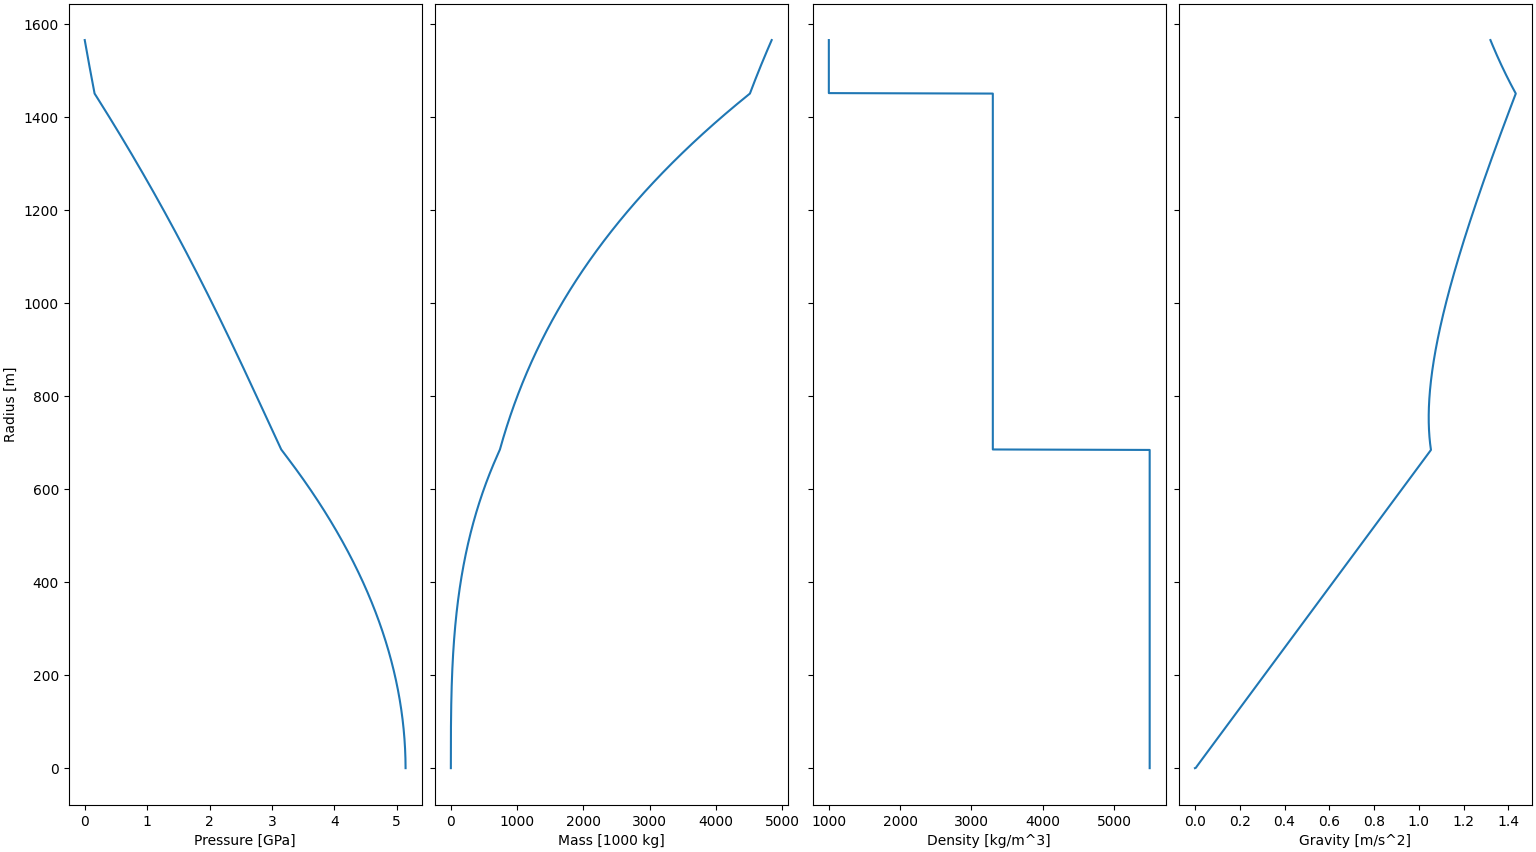
\includegraphics[width=\textwidth]{profile1.png}
	\caption{The pressure, mass, density, and gravitational acceleration of model I, plotted as a function of the radius.}
	\label{fig:profile1}
\end{figure*}
To verify the model, a few tests were done. The sensitivity of the code was checked by decreasing the initial core radius by 1 km and running the program again. Another check was done by decreasing the initial shell thickness, and two more by increasing each of the values by 1 km. All output values remained the same in each of these four cases. Even when the initial core radius is set to 0, the program eventually converges to roughly the same values as with more realistic initial conditions. Together with the fact that the functions written for the simulation were verified by comparing their outputs with analytical solutions of the equations they were made to solve, this model can be considered verified.\\
The model was validated by changing all the inputs to Earth's characteristics, as these are known with more certainty than Europa's characteristics\footnote{The thickness and density of each layer was taken from \url{http://hyperphysics.phy-astr.gsu.edu/hbase/Geophys/earthstruct.html}.}. The model accurately predicted the pressure at Earth's centre as well as the gravitational acceleration at Earth's surface. It also quite accurately predicted the size of Earth's core, but, interestingly enough, it seems to favour an unrealistically thick crust regardless of the initial conditions set. This could be a consequence of the somewhat oversimplified criteria for adjusting the core radius and crust thickness, or of the assumption that the density of each layer is homogeneous. Such an assumption should more significantly affect a model of Earth than of Europa simply because Earth is so much more massive. It can be concluded that although it is a simplified model, it is accurate and realistic enough for the purpose of this report.
\section{Thermal Effects}
To construct model II, model I is extended to include the effects of temperature on the density of each of Europa's layers. To this end, three thermal profiles are constructed, based on three centre temperature values found in literature: a minimum temperature, a maximum temperature, and a mean temperature.\\
Information about the core temperature of Europa is not easy to find. When it is mentioned in literature, it appears to be mostly speculative values, which makes sense, given the limited information available about Europa in general. Cammarano et al.\cite{cammaranoLongperiodSeismologyEuropa2006}, for example, argue that for the core to be solid, its temperature must be below 1900 K for a pure iron core, and below 1400 for an FeS core. Travis et al.\cite{travisWholemoonThermalHistory2012} propose a core temperature of 1750 K based on their simulations of the thermal history of Europa. Kuskov and Kronrod\cite{kronrodChemicalDifferentiationGalilean2006} found a temperature of 1293 degrees Celsius, or 1566 K, at the core-mantle boundary using one of their simulations. Finally, Prentice\cite{prenticeORIGINBULKCHEMICAL1999} modeled Europa with a core temperature of 1073 K.\\
% Please add the following required packages to your document preamble:
% \usepackage{graphicx}
\begin{table}[h]
	\centering
	\caption{The centre temperature values chosen as basis of the three thermal profiles for Europa.}
	\label{tab:coretemps}
		\begin{tabular}{l|l}
			\textbf{Min}  & 1073 K \\
			\textbf{Mean} & 1447 K \\
			\textbf{Max}  & 1750 K
		\end{tabular}%
\end{table}
Based on these values, three core temperatures were selected, as shown in Table \ref{tab:coretemps}. Using a linear temperature profile ranging from the core temperature to the surface temperature, chosen to be 104 K\cite{howellLikelyThicknessEuropas2021}, a density profile can be constructed using the following equation:
\begin{equation}
	\label{eq:temperature}
	\rho(T) = \rho_0(1-\alpha_T\Delta T + \frac{1}{K}\Delta p)
\end{equation}
In the above equation, $\alpha_T$ represents the thermal expansivity of the material, and K represents the bulk modulus of the material. $\rho_0$ represents a reference density. The values used in model II to calculate the density as a function of the temperature are provided in Table \ref{tab:tempeffects}.
% Please add the following required packages to your document preamble:
% \usepackage{graphicx}
\begin{table}[]
	\caption{The values used to determine the density at each point in the profile.}
	\label{tab:tempeffects}
	\resizebox{\columnwidth}{!}{%
		\begin{tabular}{|l|l|l|l|}
			\hline
			& \textbf{Core} & \textbf{Mantle} & \textbf{Shell} \\ \hline
			\textbf{Material}           & Iron sulfide  & Pyrolitic       & Water          \\ \hline
			\textbf{Density [$kg/m^3$]}   & 5500          & 3300            & 1000           \\ \hline
			\textbf{Expansivity [$K^{-1}$]} & 87e-6\cite{gronvoldThermodynamicsIronSulfides}         & 40e-6\cite{chopelasThermalExpansivityLower1992}           & -4.93e-8\cite{koyamaThermalExpansivityTwodimensional2001}       \\ \hline
			\textbf{Bulk modulus [GPa]} & 75.2\cite{terranovaPhaseStabilityThermodynamic2017}         & 130\cite{murakamiRelationshipPhysicalProperties2001}             & 10.56\cite{neumeierElasticConstantsBulk2018}          \\ \hline
		\end{tabular}%
	}
\end{table}
Equation \ref{eq:temperature} is implemented into model I by using it to update the density profile after each iteration. Because Equation \ref{eq:temperature} requires the pressure as an input, and the density profile is required to calculate the pressure profile, the first iteration is done using the same homogeneous density profile used in Model I. Aside from these things, the model works in the same way as model I.
%To construct temperature profiles, it is first necessary to determine for each layer if it is mainly convective or mainly conductive. This is done by calculating the Rayleigh number for each layer, given by the following equation:
%\begin{equation}
%	Ra = \frac{\rho\alpha g\Delta TD^3}{\kappa\eta}
%\end{equation}
%in which $\alpha$ represents the thermal expansivity of the layer, D represents the thickness of the layer, $\kappa$ the thermal diffusivity, and $\eta$ the viscosity.
\section{Results, Verification and Validation of Model II}
The results of model II are summarised in Table \ref{tab:model2results}, and the full profiles are shown in Figure \ref{fig:profile2}. In these graphs, the profiles for the minimum, mean, and maximum temperature are plotted on top of each other. The profiles are so similar to each other, though, that the difference between them is not visible in any of the graphs except for the temperature graph. To validate model II, the resulting graphs were qualitatively compared with graphs found in literature. Comparing model II to the model created by Jin and Ji\cite{jinInternalStructureModels2012} shows that the shape of the plot is very similar to that plotted by Jin and Ji. This becomes more apparent when overlaying the two figures, which is shown in Figure \ref{fig:comparison}. It is interesting to note that although the shapes of the plots are quite similar, the centre pressure obtained by model II is lower than any of Jin and Ji's models by almost 0.5 GPa. Comparing model II to the values given in Table \ref{tab:modelcomparison}, all values roughly match those found in literature.
% Please add the following required packages to your document preamble:
% \usepackage{graphicx}
\begin{table}[]
	\caption{The results of model II for the minimum core temperature, mean core temperature, and maximum core temperature.}
	\label{tab:model2results}
	\resizebox{\columnwidth}{!}{%
		\begin{tabular}{|l|l|l|l|}
			\hline
			& \textbf{Min}    & \textbf{Mean}   & \textbf{Max}    \\ \hline
			\textbf{Mass deviation}             & 0.932\% & 0.779\% & 0.928  \\ \hline
			\textbf{Centre pressure [GPa]}      & 5.11   & 5.11   & 5.10   \\ \hline
			\textbf{Gravity at surface [m/$s^2$]} & 1.32   & 1.32   & 1.32   \\ \hline
			\textbf{Core radius [km]}           & 690    & 799    & 711    \\ \hline
			\textbf{Shell thickness [km]}       & 117    & 164    & 114    \\ \hline
			\textbf{MOI deviation}          & 0.0286\% & 0.0934\% & 0.0282\% \\ \hline
			\textbf{Iterations}                 & 132    & 1      & 125    \\ \hline
		\end{tabular}%
	}
\end{table}
\begin{figure}[h]
	\centering
	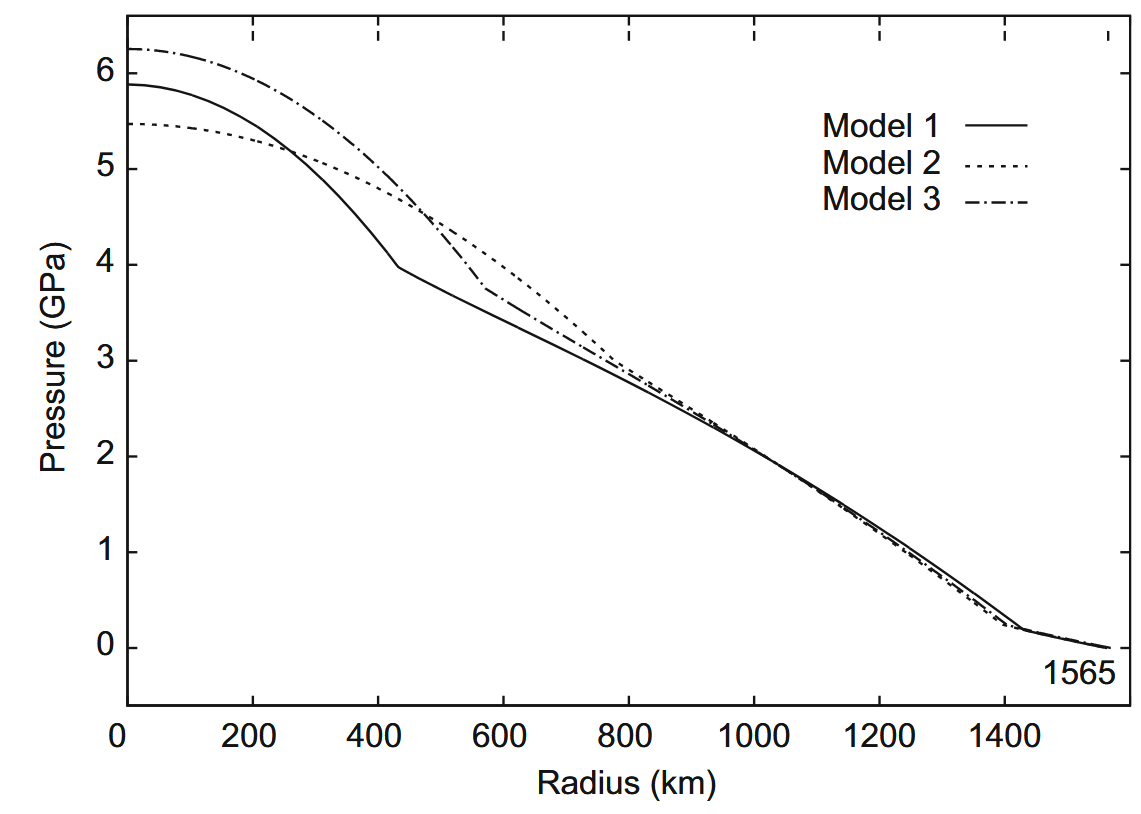
\includegraphics[width=\columnwidth]{jinjipressure.png}
	\caption{The interior pressure of Europa as determined by Jin and Ji\cite{jinInternalStructureModels2012}.}
	\label{fig:jinjipressure}
\end{figure}
\begin{figure}[h]
	\centering
	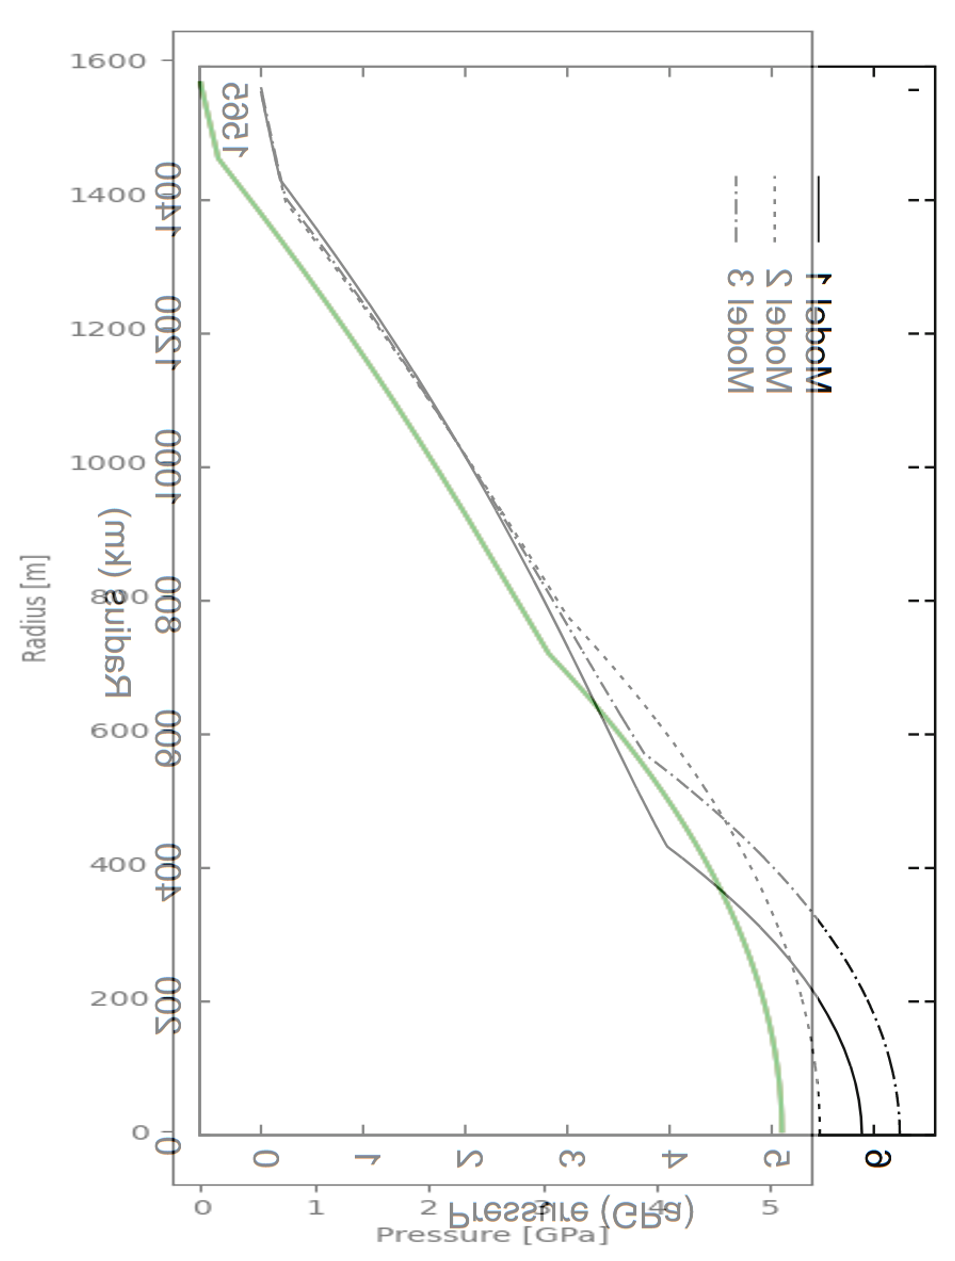
\includegraphics[width=\columnwidth]{comparison.png}
	\caption{Figure \ref{fig:jinjipressure} rotated, mirrored, and overlaid on top of the pressure graph from Figure \ref{fig:profile2}.}
	\label{fig:comparison}
\end{figure}
\begin{figure*}[h]
	\centering
	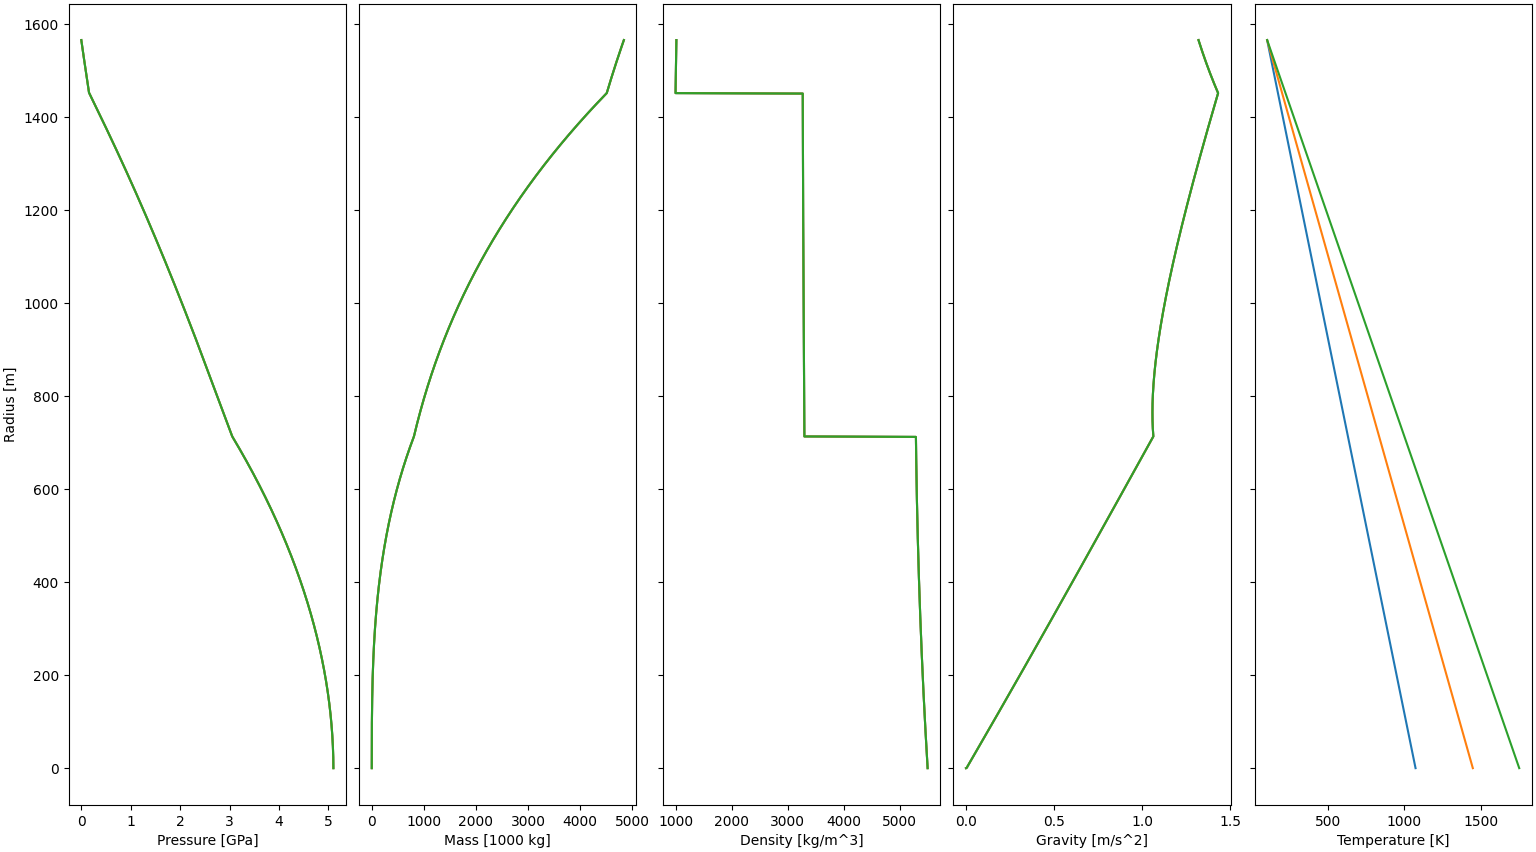
\includegraphics[width=\textwidth]{profile2.png}
	\caption{The pressure, mass, density, and gravitational acceleration of model II, plotted as a function of the radius.}
	\label{fig:profile2}
\end{figure*}
\section{Results, Verification, and Validation of Model III}
\label{sec:model3}
Unfortunately, due to problems installing the BurnMan module, model III has not been constructed yet.
\section{Comparison between models I and II}
When comparing the values found with model I with those found using model II, some interesting observations can be made. Firstly, the models predict the core of Europa to be largest at the chosen mean temperature value rather than at one of the extreme ends. At the mean temperature, the predicted core radius is 799 km, which is significantly higher than the 683 km radius found by model I. It can be concluded that choosing a good temperature profile is important for the quality of the model, as it has a large effect on the outcome.\\
It should be noted that the mean temperature model is the only one of the models that converges within one iteration. Setting a significantly different initial core radius, for example 600 km instead of the 800 km used to generate the results in Table \ref{tab:model2results}, also results in a lower core radius, namely 601 km, to which the model also converges after a single iteration. Using the same initial core radius in model I results in a radius of 649 km compared to 683 km, so it does seem that model II is more sensitive to the initial core radius value than model I.\\
The central pressures predicted by the different models are almost exactly the same, and so is the gravitational acceleration. The shell thicknesses predicted by the models are all within a few km of each other apart from, once again, the mean temperature model. This could again be because this model is sensitive to the initial core radius and/or initial shell thickness value.
\section{Conclusion}
In this report, four interior models from literature were analysed and compared to each other. Furthermore, two new models were constructed and compared to both each other and the models found in literature. These two models have shown to provide a decent first estimate for the interior profile of Europa, and they roughly agree with the models found in literature. However, there is a lot of uncertainty in the input values taken from literature. Future missions to Europa could provide more accurate data that can be used to construct more accurate models. The models themselves are quite simplified, and neglect many factors necessary to create a realistic model. In future research, these models could perhaps be expanded to include more than 3 layers, and thermal effects such as tidal heating or radiogenic heating.

\bibliographystyle{ieeetr}
\bibliography{ExportedItems.bib}

\end{document}
